\documentclass{article}
\usepackage[utf8]{inputenc}
\usepackage{graphics}
\usepackage{blindtext}
\usepackage{wrapfig}
\usepackage{graphicx}

\title{Umelá inteligencia v hrách\thanks{Semestrálny projekt v predmete Metódy inžinierskej práce, ak. rok 2021/22, vedenie: Igor Stupavský}} 

\author{Ondrej Podhorsky\\[2pt]
	{\small Slovenská technická univerzita v Bratislave}\\
	{\small Fakulta informatiky a informačných technológií}\\
	{\small \texttt{xpodhorsky@stuba.sk}}
	}

\date{\small 6. november 2022}

\begin{document}

\maketitle

\begin{abstract}
\ldots
\end{abstract}

Cieľom tohto článku je priblížiť použitie a možnosti použitia umelej inteligencie v video hernom priemysle, ktorý sa v súčasnosti dostáva do popredia v zábavnom priemysle. V roku 2022 by mal podľa očakávaní mať výnos 197 biliónov dolárov, čo by ho radilo napríklad pred hudobný alebo filmový priemysel. Dlhodobo sa snažili najpoprednejšie štúdia vyvíjať hry s dôrazom  na grafickú realistickosť. No v podstate tento ciel už bol dosiahnutý a preto sa snažia implementovať iné technológie do svojich hier, ktorými by sa dal obohatiť video herný zážitok, zjednodušiť ich vývin či testovanie hier.
\clearpage
\section{Úvod}

Aplikácie umelej inteligencie nie je jednoduchá. Čelí množstvu problémov ale zároveň má obrovský potenciál posunúť hry ďalej. Prvá časť bude obsahovať informácie o disciplíne, ktorú použitie umelej iteligencie definovalo. V ďalších častiach sa bude písať o aspektoch hry, ako je napríklad tvorba a fungovanie nehráčských postáv a jej limitáciám, vylepšením tvorby herného zážitku implentovaním umelej inteligencie do herných mechaník a generovaním obashu pre zjednodušenie práce herných vývojárov.

\begin{figure}{h}
\centering
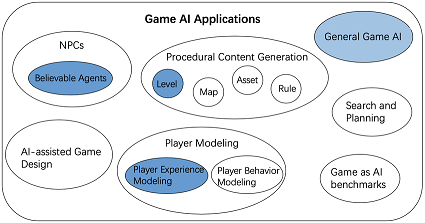
\includegraphics[width=\textwidth]{Game-AI-Applications.png}
\end{figure}

\section{Hry ako testovacie prostredie}

\section{Nehráčske postavy}

Nehráčske postavy sú neodmysliteľnou časťou hier od nepamäti, napríklad duchovia z hry Pac-Man(1980). Sú to prevažne charaktery, ktoré ovláda počítač po prípade hráč. No v súčasnosti je to časť hry, ktorá sa často prehliada a priorita sa hlavne prikladá na grafickú stránku hier. Umelá inteligencia má potenciál tento problém vyriešiť. Momentálne sa prevažne používajú primitívne postupy vytvorené ešte v 90tich rokoch, ktoré sú napríklad pathfinding,finite state machines alebo komplexnejšie ako je napríklad Monte Carlo Tree Search. Vývojári v posledných dekádach len zväčšujú merítko v akom sú tieto koncepty využívané.

\subsection{Limitácie}

Hlavnými obmedzeniami sú nedostatočné výpočtové prostriedky dostupné pre bežného používateľa. Tak tiež nepredvídateľnosť takýchto charakterov by vytvárala chaos a práve naopak by ešte viac znížila pocit prirodzeného správania a podkopala tak video herný zážitok.

\section{Tvorba herného zážitku}

\section{Generovanie herného obsahu}
\section{Záver}

\bibliography{literatura}
\bibliographystyle{plain}
\end{document}
